%===============================================================================
% Zentrale Layout-Angaben und Befehle
%===============================================================================
%
% Für bessere Sicht von falschen Umbrüchen die Option draft benutzen.
% Dadurch können aber die eingebundenen Bilder nicht sichtbar sein.
\documentclass[a4paper, 12pt]{article}
%
% Hier zunächst die benötigten Packages
\usepackage[utf8]{inputenc}
\usepackage{fancyhdr}
\usepackage[T1]{fontenc}
\usepackage{ae}
\usepackage{listings}
\usepackage{color}
\usepackage{wrapfig}
\usepackage[printonlyused]{acronym}
\usepackage{url}
\usepackage[hypertexnames=false]{hyperref}
\usepackage{fmtcount}
\usepackage[section]{placeins}
\usepackage{tabularx}
\usepackage{amsmath}
\usepackage{nameref}
%
% Einbindung des Grafik-Pakets
\ifx\pdfoutput\undefined
	\usepackage[dvips]{graphicx}
\else
	\usepackage[pdftex]{graphicx}
\pdfcompresslevel=9
\pdfpageheight=297mm
\pdfpagewidth=210mm
\fi
\usepackage[colorinlistoftodos,prependcaption,textsize=tiny]{todonotes}
%
% Page-Layout
\setlength\headheight{14pt}
\setlength\topmargin{-15,4mm}
\setlength\oddsidemargin{-0,4mm}
\setlength\evensidemargin{-0,4mm}
\setlength\textwidth{160mm}
\setlength\textheight{252mm}
%
% Absatzeinstellungen
\setlength\parindent{0mm}
\setlength\parskip{2ex}
%
% dont break math space
\binoppenalty=10000
\relpenalty=10000
%
% Kopf- und Fusszeile
\pagestyle{fancy}
\fancyhf{} % alles löschen
\fancyhead[LO]{\footnotesize\sc\nouppercase{\leftmark}}
\fancyfoot[LO]{\footnotesize\sc Distributed Systems Group}
\fancyfoot[RO]{\thepage}
\renewcommand{\headrulewidth}{0pt}
\renewcommand{\footrulewidth}{0pt}
%
% Bessere Fehlermeldungen
\errorcontextlines=999
%
% Anweisung zur Erstellung der Titelseite
% #1 Bachelorarbeit || Masterarbeit
% #2 = Studiengang
% #3 = Titel der Arbeit
% #4 = Autor
% #5 = Abgabedatum
\renewcommand{\maketitle}[6]
{
\pagenumbering{Alph}
\begin{titlepage}
\centering
\begin{minipage}[t]{16cm}
\begin{minipage}{3cm}
    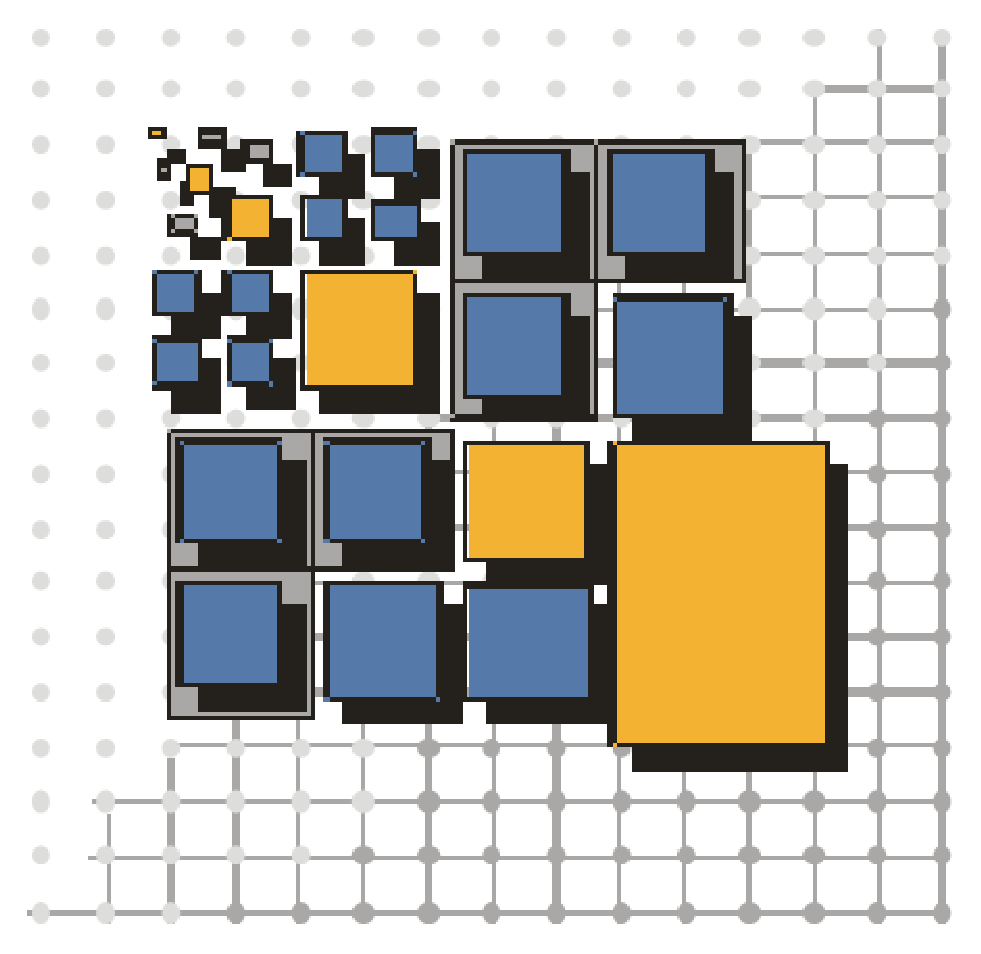
\includegraphics[height=26mm]{includes/vs-logo}
\end{minipage}
\hfill
\begin{minipage}{9cm}
  \centering
    University of Bamberg\\[12pt]
    {\Large Distributed Systems Group}
\end{minipage}
\hfill
\begin{minipage}{3cm}
    
\includegraphics[height=26mm]{includes/UB-Logo-neu_blau-cmyk}
\end{minipage}
\end{minipage}\\[130pt]
{\LARGE #1}\\[124pt]
With the topic:\\[24pt]
{\Huge #2}\\[60pt]
\vfill
\begin{minipage}{\textwidth}
\center
Submitted by:\\
{\Large #3\\[12pt]}
Supervisor:\\
{#5\\[12pt]}
Examiner:\\
#6\\[12pt]
Date of submission:\\
#4\\
\end{minipage}
\end{titlepage}
}

%
% Wird für Hintergrund von Codelistings benötigt
\definecolor{hellgrau}{gray}{0.9}
%
\lstdefinelanguage{JavaScript}{
	keywords={typeof, new, true, false, catch, function, return, null, catch, switch, var, if, in, while, do, else, case, break},
	ndkeywords={class, export, boolean, throw, implements, import, this},
	sensitive=false,
	comment=[l]{//},
	morecomment=[s]{/*}{*/},
	morestring=[b]',
	morestring=[b]"
}
% Einstellungen für Java-Code
\lstdefinestyle{javaStyle}{%
	basicstyle=\small,%
	backgroundcolor=\color{hellgrau},%
	keywordstyle=\bfseries,%
	showstringspaces=false,%
	numbers=left,%
	numberstyle=\footnotesize,%
	stepnumber=1,%
	numbersep=3pt,%
	extendedchars=true,%
	xleftmargin=2em,%
	lineskip=-1pt,%
	tabsize=4,%
	language=Java,
	breaklines,%
	identifierstyle=\ttfamily,
}
% set default to java, explicitly set to others when needed
\lstset{style=javaStyle}
%
% neues environment für Java-Sourcecode
% #1 = "caption={Hier eigene Überschrift}, label={Hier eigenes Label}"
\lstnewenvironment{javacode}[1][]{%
\lstset{style=javaStyle,#1}%
}{}
%
% Befehl zum Einbinden von Java-Sourcecode aus Datei
% #1 = Dateiname relativ zu src-Verzeichnis
% #2 = Überschrift
% #3 = Label
\newcommand{\javafile}[3]{%
   \lstinputlisting[%
     caption={#2},%
     label={#3},%
     style=javaStyle,
     captionpos=b]{src/#1}%
}
%
% Einbindung eines Bildes
% #1 = Name des Bildes ohne Endung relativ zu images-Verzeichnis
% #2 = Caption
% #3 = label für \ref-Verweise
% #4 = Breite des Bildes im Dokument in % der breite
\newcommand{\asfigure}[4]{%
  \begin{figure}[htb]%
    \begin{center}%
      \includegraphics[width=#4\textwidth]{images/#1}%
      \vskip -0.3cm%
      \caption{#2}%
      \vskip -0,2cm%
      \label{#3}%
    \end{center}%
  \end{figure}%
}
%
% Umgebung für Fliesstext um Grafik
% #1 = Ausrichtung: r, l, i, ...
% #2 = Breite des Bildes in cm
% #3 = Name des Bildes ohne Endung relativ zu images-Verzeichnis
% #4 = Beschriftung
% #5 = label für \ref-Verweise
\newcommand{\textflow}[5]{%
\begin{wrapfigure}{#1}{#2cm}%
\includegraphics[width=#2cm]{images/#3}%
\caption{#4}%
\label{#5}%
\end{wrapfigure}%
}
%%%
\makeatletter
\let\orgdescriptionlabel\descriptionlabel
\renewcommand*{\descriptionlabel}[1]{%
	\let\orglabel\label
	\let\label\@gobble
	\phantomsection
	\edef\@currentlabel{#1}%
	%\edef\@currentlabelname{#1}%
	\let\label\orglabel
	\orgdescriptionlabel{#1}%
}
\makeatother

%%% Local Variables:
%%% mode: latex
%%% TeX-master: t
%%% End:
